\chapter{Example of application on a regional turboprop}
\label{ch3}

\begin{figure}[htbp]
\centering
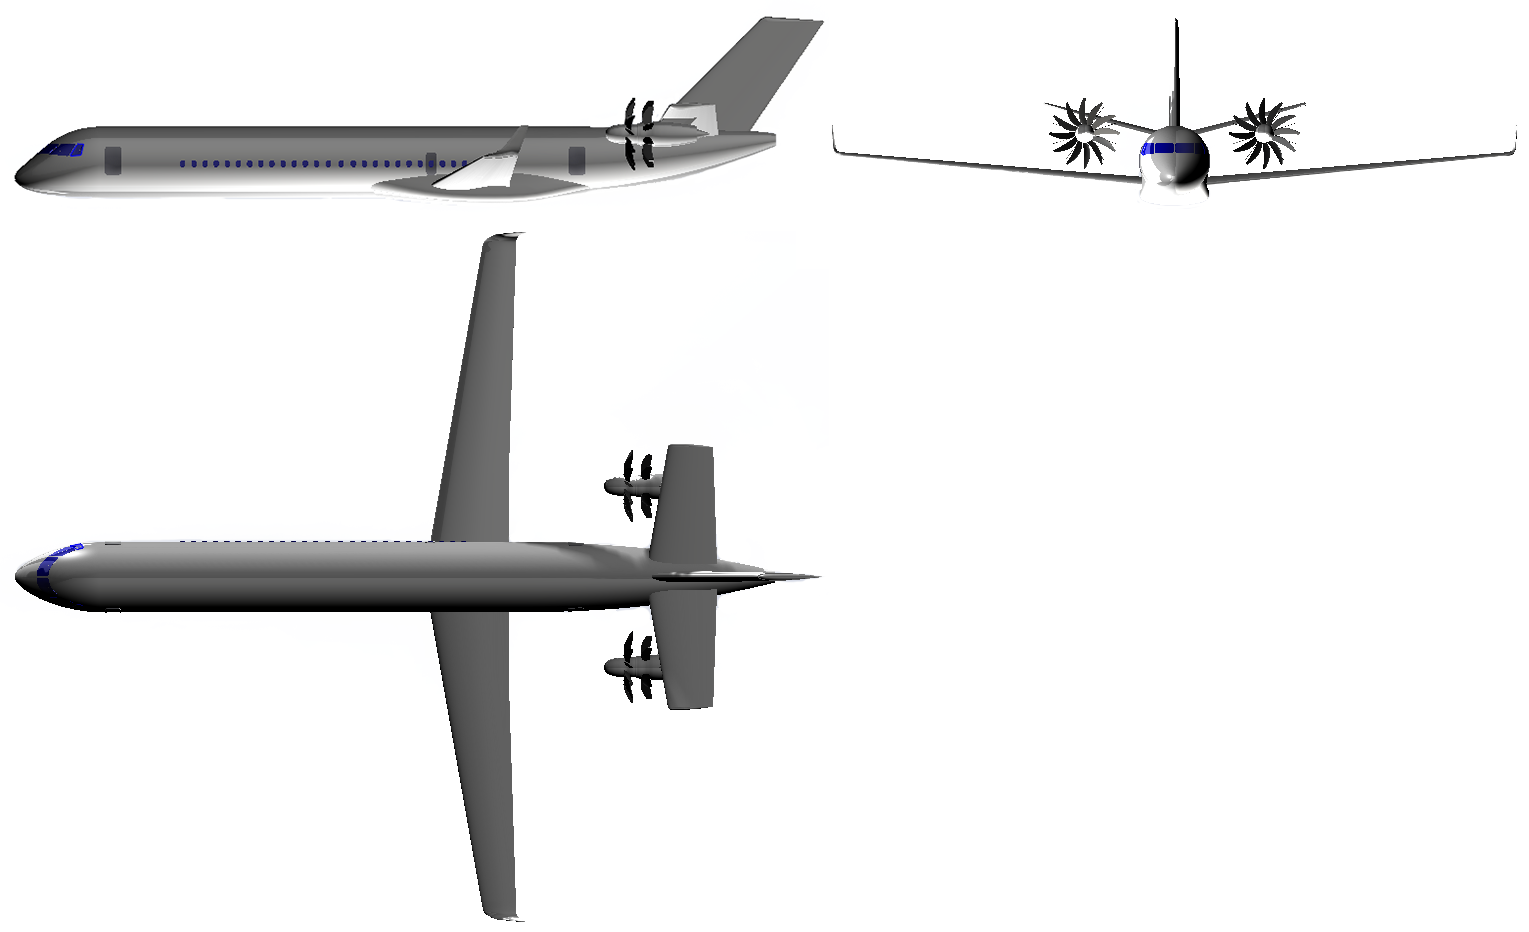
\includegraphics[width=\textwidth]{Immagini/Capitolo3/IRON}
\caption{Three views of the aircraft}
\end{figure}

\newpage

\begin{table}[H]
\centering
\caption{Aircraft data}
\begin{tabular}{ccc}
\toprule
Variable & SI units & USCS units \\
\midrule
\CDo & $\SI{0.03035}{}$ & ---\\
\xcgadim & $\SI{0.1}{}$ & ---\\
SSM & $\SI{-0.080}{}$ & ---\\
\bottomrule
\end{tabular}
\end{table}

\begin{table}[H]
\centering
\caption{Flight conditions}
\begin{tabular}{ccc}
\toprule
Variable & SI units & USCS units \\
\midrule
\alphaB & $\SI{0}{rad}$ & $\SI{0}{deg}$ \\
\CLift & $\SI{0.650}{}$ & --- \\
$M$ & $\SI{0.640}{}$ & ---\\
\bottomrule
\end{tabular}
\end{table}

\begin{table}[H]
\centering
\caption{Wing related parameters}
\begin{tabular}{ccc}
\toprule
Variable & SI units & USCS units \\
\midrule
\SW & $\SI{98.60}{m^2}$ & $\SI{1061.32}{ft^2}$ \\
\bW & $\SI{34.34}{m}$ & $\SI{112.66}{ft}$ \\
\ARW & $\SI{11.961}{}$ & --- \\
\lambdaW & $\SI{0.383}{}$ & --- \\
$\Lambda_{c/4, \text W}$ & $\SI{0.10159}{rad}$ & $\SI{5.821}{deg}$ \\
$\Lambda_{c/2, \text W}$ & $\SI{0.02755}{rad}$ & $\SI{1.578}{deg}$ \\
\GammaW & $\SI{0.09599}{rad}$ & $\SI{5.5}{deg}$ \\
\epsW & $\SI{-0.03491}{rad}$ & $\SI{-2}{deg}$ \\
\CLalphaW & $\SI{6.342}{rad^{-1}}$ & $\SI{0.11068}{deg^{-1}}$ \\
\ZW & $\SI{1.33}{m}$ & $\SI{4.36}{ft}$ \\
\etaailin & $\SI{0.78}{}$ & --- \\
\etaailout & $\SI{0.95}{}$ & --- \\
$\overline c_\text{a}/\overline c_{\text {W (at aileron)}}$ & $\SI{0.32}{}$ & --- \\
\tauail & $\SI{0.530}{}$ & --- \\
\bottomrule
\end{tabular}
\end{table}

\begin{table}[H]
\centering
\caption{Fuselage related parameters}
\begin{tabular}{ccc}
\toprule
Variable & SI units & USCS units \\
\midrule
$S_{\mathrm P \rightarrow \mathrm V}$ & $\SI{6.77}{m^2}$ & $\SI{72.85}{ft^2}$ \\
\SBside & $\SI{108.46}{m^2}$ & $\SI{1167.45}{ft^2}$ \\
$Re_\textrm B$ & 2.35E8 & --- \\
$d_{\text W,\text B}$ & $\SI{3.54}{m}$ & $\SI{11.60}{ft}$ \\
$d_{\text W,\text H}$ & $\SI{2.46}{m}$ & $\SI{8.07}{ft}$ \\
$d$ & $\SI{3.56}{m}$ & $\SI{11.69}{ft}$ \\
$l_\text B$ & $\SI{38.04}{m}$ & $\SI{124.80}{ft}$ \\
$w_\text{max}$ & $\SI{3.51}{m}$ & $\SI{11.52}{ft}$ \\
$Z_\text{max}$ & $\SI{3.56}{m}$ & $\SI{11.69}{ft}$ \\
$Z_1$ & $\SI{3.56}{m}$ & $\SI{11.69}{ft}$ \\
$Z_2$ & $\SI{3.46}{m}$ & $\SI{11.34}{ft}$ \\
$r_1$ & $\SI{2.60}{m}$ & $\SI{8.53}{ft}$ \\
\bottomrule
\end{tabular}
\end{table}

\begin{table}[H]
\centering
\caption{Horizontal tail related parameters}
\begin{tabular}{ccc}
\toprule
Variable & SI units & USCS units \\
\midrule
\SH & $\SI{39.91}{m^2}$ & $\SI{429.59}{ft^2}$ \\
\bH & $\SI{13.04}{m}$ & $\SI{42.78}{ft}$ \\
\ARH & $\SI{4.261}{}$ & --- \\
\lamH & $\SI{0.624}{}$ & --- \\
$\Lambda_{c/4, \text H}$ & $\SI{0.07485}{rad}$ & $\SI{4.286}{deg}$ \\
$\Lambda_{c/2, \text H}$ & $\SI{-0.02633}{rad}$ & $\SI{-1.509}{deg}$ \\
\GammaH & $\SI{0.26180}{rad}$ & $\SI{15}{deg}$ \\
\epsH & $\SI{0}{rad}$ & $\SI{0}{deg}$ \\
\CLalphaH & $\SI{4.261}{rad^{-1}}$ & $\SI{0.07437}{deg^{-1}}$ \\
\etaH & $\SI{0.8}{}$ & ---\\
\bottomrule
\end{tabular}
\end{table}

\begin{table}[H]
\centering
\caption{Vertical tail related parameters}
\begin{tabular}{ccc}
\toprule
Variable & SI units & USCS units \\
\midrule
\SV & $\SI{24.45}{m^2}$ & $\SI{263.18}{ft^2}$ \\
\bV & $\SI{5.78}{m}$ & $\SI{18.96}{ft}$ \\
\lamV & $\SI{0.640}{}$ & --- \\
\XV & $\SI{13.17}{m}$ & $\SI{43.21}{ft}$ \\
\ZV & $\SI{1.52}{m}$ & $\SI{4.99}{ft}$ \\
\CLalphaV & $\SI{2.079}{rad^{-1}}$ & $\SI{0.03629}{deg^{-1}}$ \\
\etaV & $\SI{0.9}{}$ & ---\\
\etarudin & $\SI{0}{}$ & --- \\
\etarudout & $\SI{0.9}{}$ & --- \\
$\overline c_\text{r}/\overline c_{\text {V}}$ & $\SI{0.35}{}$ & --- \\
\taurud & $\SI{0.562}{}$ & --- \\
\XR & $\SI{15.21}{m}$ & $\SI{49.90}{ft}$ \\
\ZR & $\SI{4.12}{m}$ & $\SI{13.52}{ft}$ \\
\bottomrule
\end{tabular}
\end{table}

\begin{table}[H]
\centering
\caption{Outcome parameters from lateral-directional calculations -- Steady coefficients}
\begin{tabular}{ccc}
\toprule
Variable & SI units & USCS units \\
\midrule
\CYzero & $\SI{0}{}$ & ---\\
\CYbetaW & $\SI{-0.032}{rad^{-1}}$ & $\SI{-0.00056}{deg^{-1}}$\\
\CYbetaB & $\SI{-0.154}{rad^{-1}}$ & $\SI{-0.00269}{deg^{-1}}$\\
\CYbetaH & $\SI{-0.056}{rad^{-1}}$ & $\SI{-0.00098}{deg^{-1}}$\\
\CYbetaV & $\SI{-0.533}{rad^{-1}}$ & $\SI{-0.00930}{deg^{-1}}$\\
\CYbeta & $\SI{-0.774}{rad^{-1}}$ & $\SI{-0.01351}{deg^{-1}}$\\
\CYdeltaa & $\SI{0}{rad^{-1}}$ & $\SI{0}{deg^{-1}}$ \\
\CYdeltar & $\SI{0.251}{rad^{-1}}$ & $\SI{0.00438}{deg^{-1}}$\\
\CLzeroRoll & $\SI{0}{}$ & ---\\
\CLbetaWB & $\SI{-0.056}{rad^{-1}}$ & $\SI{-0.00098}{deg^{-1}}$\\
\CLbetaH & $\SI{-0.024}{rad^{-1}}$ & $\SI{-0.00042}{deg^{-1}}$\\
\CLbetaV & $\SI{-0.024}{rad^{-1}}$ & $\SI{-0.00042}{deg^{-1}}$\\
\CLbeta & $\SI{-0.104}{rad^{-1}}$ & $\SI{-0.00182}{deg^{-1}}$\\
\CLdeltaa & $\SI{-0.052}{rad^{-1}}$ & $\SI{-0.00091}{deg^{-1}}$\\
\CLdeltar & $\SI{0.030}{rad^{-1}}$ & $\SI{0.00052}{deg^{-1}}$\\
\CNzeroYaw & $\SI{0}{}$ & ---\\
\CNbetaBody & $\SI{-0.167}{rad^{-1}}$ & $\SI{-0.00292}{deg^{-1}}$\\
\CNbetaV & $\SI{0.205}{rad^{-1}}$ & $\SI{0.00357}{deg^{-1}}$\\
\CNbeta & $\SI{0.038}{rad^{-1}}$ & $\SI{0.00065}{deg^{-1}}$\\
\CNdeltaa & $\SI{0}{rad^{-1}}$ & $\SI{0}{deg^{-1}}$\\
\CNdeltar & $\SI{-0.111}{rad^{-1}}$ & $\SI{-0.00194}{deg^{-1}}$\\
\bottomrule
\end{tabular}
\end{table}

\begin{table}[H]
\centering
\caption{Outcome parameters from lateral-directional calculations -- Unsteady coefficients}
\begin{tabular}{ccc}
\toprule
Variable & SI units & USCS units \\
\midrule
\CYprate & $\SI{-0.047}{rad^{-1}}$ & $\SI{-0.00082}{deg^{-1}}$\\
\CYrrate & $\SI{0.409}{rad^{-1}}$ & $\SI{0.00714}{deg^{-1}}$\\
\CLprateWB & $\SI{-0.522}{rad^{-1}}$ & $\SI{-0.00911}{deg^{-1}}$\\
\CLprateH & $\SI{-0.009}{rad^{-1}}$ & $\SI{-0.00016}{deg^{-1}}$\\
\CLprateV & $\SI{-0.002}{rad^{-1}}$ & $\SI{-0.00005}{deg^{-1}}$\\
\CLprate & $\SI{-0.533}{rad^{-1}}$ & $\SI{-0.00932}{deg^{-1}}$\\
\CLrrateW & $\SI{0.175}{rad^{-1}}$ & $\SI{0.00305}{deg^{-1}}$\\
\CLrrateV & $\SI{0.018}{rad^{-1}}$ & $\SI{0.00031}{deg^{-1}}$\\
\CLrrate & $\SI{0.193}{rad^{-1}}$ & $\SI{0.00336}{deg^{-1}}$\\
\CNprateW & $\SI{-0.095}{rad^{-1}}$ & $\SI{-0.00166}{deg^{-1}}$\\
\CNprateV & $\SI{0}{rad^{-1}}$ & $\SI{0}{deg^{-1}}$\\
\CNprate & $\SI{-0.095}{rad^{-1}}$ & $\SI{-0.00166}{deg^{-1}}$\\
\CNrrateW & $\SI{-0.017}{rad^{-1}}$ & $\SI{-0.00029}{deg^{-1}}$\\
\CNrrateV & $\SI{0.084}{rad^{-1}}$ & $\SI{0.00146}{deg^{-1}}$\\
\CNrrate & $\SI{0.067}{rad^{-1}}$ & $\SI{0.00117}{deg^{-1}}$\\
\bottomrule
\end{tabular}
\end{table}